%!TEX root=finmath1.tex
\chapter{Подразумеваемая волатильность}
\label{ch:iv}
\chaptertoc

\emph{Подразумеваемая волатильность} "--- это такое значение параметра волатильности $\sigma$, которое рынок закладывает в цены опционов.
В этой лекции мы обсудим метод вычисления подразумеваемой волатильности из рыночных цен европейских опционов, а также увидим, что в реальных данных она различается для опционов с различными страйками и временем экспирации.
Этот факт, в частности, означает, что модель \bs\ на практике не верна.

\section{Понятие подразумеваемой волатильности}
\subsection{Определение и комментарии}

Далее мы будем работать с ценами европейских опционов колл и пут, вычисляемыми по формуле Блэка.
В этой формуле цена зависит от 5 аргументов: время до экспирации $T$ (текущий момент времени $t$ будет всегда считаться нулевым), страйк $K$, $T$-форвардная цена $F$, цена бескупонной облигации $B$ c погашением в момент $T$ и волатильность $\sigma$.
Значения первых четырех аргументов известны либо из спецификации самого опциона ($T$, $K$), либо из рыночных данных ($F$, $B$ "--- ниже будет объяснено, как их получить).
Значение волатильности $\sigma$ является модельным параметром и должно быть оценено.

С другой стороны, рыночные цены опционов известны (из котировок на бирже), поэтому на формулу Блэка 
\begin{equation}
\label{iv:equation}
\VC = \VC(T,K,F,B,\sigma) \qquad(\text{или}\ \VP = \VP(T,K,F,B,\sigma))
\end{equation}
можно посмотреть как на уравнение, в котором $\sigma$ является единственной неизвестной величиной.

\begin{definition}
\emph{Подразумеваемой} (также \emph{предполагаемой}, \emph{вмененной}, \emph{implied volatility}) \emph{волатильностью} $\hat\sigma$ называется такое значение параметра $\sigma$, что при подстановке его в формулу Блэка, цена опциона, вычисленная по этой формуле, совпадает с рыночной ценой.
\end{definition}

Таким образом, $\hat\sigma$ "--- это значение параметра волатильности, которое <<рынок закладывает>> в расчет цены опциона.

Эмпирическим фактом, наблюдаемым для всех активов, является то, что значение подразумеваемой волатильности оказывается разным для различных опционов на один и тот же базовый актив.
В качестве примера на рис.~\ref{11:f:iv} показаны подразумеваемые волатильности опционов на индекс S\&P 500.
Четко видна зависимость подразумеваемой волатильности и от $T$, и от $K$.

\begin{figure}[h]
\centering
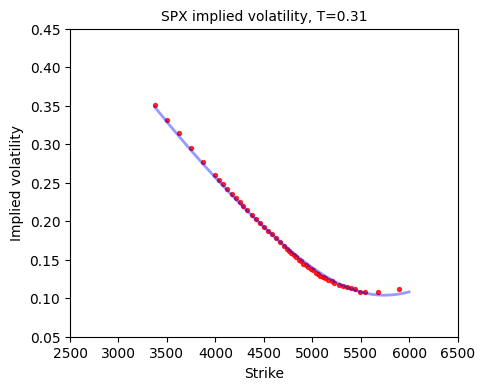
\includegraphics[height=3.7cm]{pic/iv-3m.png}
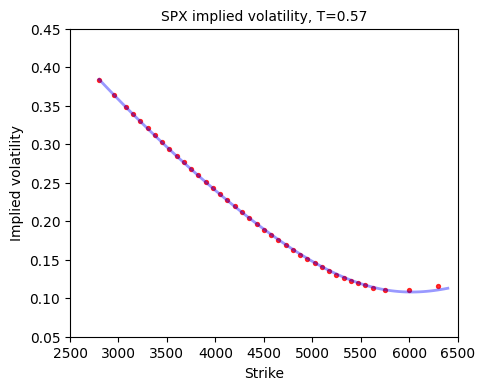
\includegraphics[height=3.7cm]{pic/iv-6m.png}
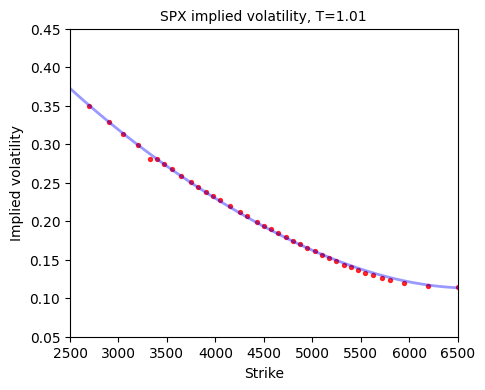
\includegraphics[height=3.7cm]{pic/iv-1y.png}
\caption{Подразумеваемые волатильности опционов на индекс S\&P 500 (данные на 6.03.2024). Три графика соответствуют трем разным значениям времени до экспирации.}
\label{11:f:iv}
\end{figure}

Это обстоятельство, в частности, означает что модель модель \bs\ на практике не верна: если бы цены всех опционов на один и тот же базовый актив вычислялись по формуле Блэка (или \bs), то $\hat\sigma$ была бы одинаковой для всех значений $T,K$ и равнялась бы параметру $\sigma$ геометрического броуновского движения.

Тем не менее, это не означает, что модель Блэка--Шоулза не нужна.
На самом деле, модель \bs\ используется для \emph{взаимнооднозначного преобразования из цен опционов в подразумеваемую волатильность}.

Оказывается, что с подразумеваемой волатильностью гораздо удобнее работать, чем с ценами опционов, так как на цену оказывают влияние еще и параметры $T,K,F,B$, в то время как волатильность очищена от этих факторов. 
Кроме того, для трейдеров значение волатильности гораздо информативнее отражает насколько дорог или дешев опцион, чем сами цены: из фразы <<волатильность опциона 50\%>> качественно понятно, что опцион дорогой, даже если не называть базовый актив; а из фразы <<цена опциона 10 долларов>> ничего не ясно без указания остальных параметров.
Наконец, совокупность значений подразумеваемой волатильности (так называемая \emph{поверхность волатильности} "--- см.~далее) используется для подгонки параметров более продвинутых моделей цен активов и является важнейшим <<входным параметром>> для них. 

\begin{remark}
Можно также вычислить \emph{историческую волатильность} "--- по прошлым ценам рискового актива статистически оценить коэффициент $\sigma$ геометрического броуновского движения.
Историческая волатильность качественно отличается от подразумеваемой в том, что, во-первых, историческая волатильность <<смотрит>> в прошлое, а подразумеваемая "--- в будущее. Во-вторых, историческая волатильность "--- это число, в то время как подразумеваемая волатильность "--- это функция от страйка и времени до экспирации опциона.
\end{remark}

Докажем полезный вспомогательный результат, который показывает, что подразумеваемая волатильность европейских опционов колл и пут совпадает.

\begin{proposition}
Если на рынке выполняется паритет цен колл-пут%
\footnote{Напомним, что паритет цен колл-пут выполняется в любой безарбитражной теоретической модели.
В реальности он тоже обычно выполняется (с точностью до погрешности, возникающей из-за транзакционных издержек).}
$($т.е.\ $\VC - \VP = B(F-K)$$)$, то значение $\hat\sigma$, вычисленное для опциона колл, совпадает со значением $\hat\sigma$, вычисленным для опциона пут с таким же страйком и временем до экспирации.
\end{proposition}

\begin{proof}
Пусть $\hat\sigma_c$ "--- подразумеваемая волатильность опциона колл, а $\hat\sigma_p$ "--- подразумевая волатильность опциона пут с такими же $T$ и $K$.
Предположим, от противного, что $\hat\sigma_c\neq \hat\sigma_p$. 

Для любого $\sigma \neq \hat\sigma_p$ имеем $\VP(\sigma) \neq \VP(\hat\sigma_p)$ так как функция $\VP$ строго возрастает по $\sigma$, что следует из положительности ее производной по $\sigma$. 
Но так как $\VC(\hat\sigma_c) - \VP(\hat\sigma_c) = B(F-K)$ из-за того, что паритет колл-пут выполняется в модели \bs, то $\VC(\hat\sigma_c) - \VP(\hat\sigma_p) \neq B(F-K)$.
В левой части здесь стоит разность рыночных цен опционов колл и пут (по определению подразумеваемой волатильности), поэтому получается, что на рынке паритет колл-пут не выполнен. 
Противоречие.
\end{proof}

\begin{definition}
\label{iv:d:surface}
Для заданного базового актива \emph{поверхностью подразумеваемой волатильности}  называется функция $\hat\sigma(T,K)$ с аргументами $T,K> 0$, выражающая зависимость подразумеваемой волатильности от времени до экспирации  и страйка.

\emph{Улыбкой подразумеваемой волатильности} для заданного времени $T>0$ называется функция $K\mapsto\sigma(T,K)$, \te\ одно сечение поверхности волатильности.
\end{definition}

Далее для краткости будем говорить просто <<поверхность волатильности>> или <<улыбка полатильности>>, опуская слово <<подразумеваемой>>.

\begin{remark}
Величина $T$ обычно выражается в годах, $K$ "--- в единицах валюты, а $\hat\sigma$ "--- безразмерная величина или выражается в процентах.
Типичные значения волатильности "--- от 0.1 до 0.5, в зависимости от актива, параметров $T,K$ опциона и ожидания риска у трейдеров.
При изменении масштаба по времени в $s$ раз волатильность следует изменить в $\sqrt{s}$ раз, \te, например, при выражении времени в месяцах типичные значения $\hat\sigma$ будут от $0.1/\sqrt{12}$ до $0.5/\sqrt{12}$.
\end{remark}

\begin{remark}
Строго говоря, волатильность $\sigma\hat(T,K)$, вычисленная из рыночных цен опционов, еще не является функцией, так как на рынке имеется лишь конечное число комбинаций $T$ и $K$ для торгуемых опционов.
Для того, чтобы получить функцию, нужно провести интерполяцию и экстраполяцию данных.
Далее мы будем считать, что эти операции уже проведены (как это правильно сделать "--- отдельная задача, которая в курсе не рассматривается).
\end{remark}


\subsection{Необходимое и достаточное условие существования подразумеваемой волатильности}
Далее будем считать, что $T>0$ и $K>0$.

\begin{proposition}
\label{iv:p:existence}
Подразумеваемая волатильность существует (\te\ уравнение \eqref{iv:equation} имеет единственное решение $\hat\sigma$) тогда и только тогда, когда
\begin{equation}
\label{iv:call-bounds}
B(F-K)^+ < \VC < BF,
\end{equation}
или, эквивалентно,
\begin{equation}
\label{iv:put-bounds}
B(K-F)^+ < \VP < BK
\end{equation}
\end{proposition}

\begin{proof}
Докажем только утверждение для опционов колл, для пут оно доказываетя аналогично.
Зафиксируем $T,K,F,B$ и будем рассматривать цену опциона колл как непрерывную функцию $V(\sigma) = \VC(T,K,F,B,\sigma)$.

Заметим, что $V$ строго возрастает, так как $V'(\sigma)>0$ для всех $\sigma>0$ (это свойство  положительности веги опциона; см.~раздел \ref{9:ss:greeks} в лекции \ref{ch:bs}).
Кроме того, 
\[
\lim_{\sigma\to\infty} V(\sigma) = BF, \qquad
\lim_{\sigma\to 0} V(\sigma) = \begin{cases}
B(F-K), &f > K,\\
0, &f\le K,
\end{cases}
\]
в чем нетрудно убедиться, переходя к пределу в формуле Блэка.
Теперь видно, что доказываемое утверждение следует из теоремы о промежуточном значении строго монотонной непрерывной функции.
\end{proof}

Отметим, что ограничения \eqref{iv:call-bounds} и \eqref{iv:put-bounds} должны выполняться в любой безарбитражной модели, а не только в модели \bs, что делает возможным вычисление подразумеваемой волатильности для любых (безарбитражных) рыночных данных, не далая конкретных предположений о модели рынка.

(Упражнение: покажите, что если $\VC<B(F-K)^+$ или $\VC> BF$, то можно построить арбитражную возможность; если дополнительно предположить, что цена $S_T$ принимает значения в любом интервале $(a,b)\subset\R_+$ с положительной вероятностью, то арбитражная возможность найдется и в случаях $\VC=B(F-K)^+$ и $\VC=BF$.
Аналогично для опционов пут.)




\section{Вычисление подразумеваемой волатильности}

\subsection{Какие данные использовать?}

Задача вычисления подразумеваемой волатильности состоит в том, чтобы для набора времен исполнения и страйков $(T_i,K_i)$ вычислить значения $\hat\sigma_i = \hat\sigma(T_i,K_i)$. 

Для каждой пары $(T_i,K_i)$, как правило, в рыночных данных имеются как минимум четыре цены: цены бид и аск%
\footnote{\emph{Бид} (bid) -- лучшая заявка на покупку в стакане заявок (с наиболее дорогой ценой), \emph{аск} (ask) -- лучшая заявка на продажу (с наиболее дешевой ценой). Цена бид всегда меньше цены аск.
Если инструмент неликвидный, то стакан заявок может содержать только одну из цен бид/аск или вообще быть пустым.}
опционов колл и цены бид и аск опционов пут; также обычно присутствуют цены последних сделок (если сделки были).
На практике для вычисления $\hat\sigma$ применяются следующие соображения.

\begin{itemize}
\item Используют только опционы АTMF и OTMF%
\footnote{
ATMF (at-the-money forward, опцион \emph{на} деньгах) -- опцион со страйком равным форвардной цене, $K=F$.
OTMF (out-of-the-money forward, опцион \emph{вне} денег) -- опцион колл с $K>F$ или опцион пут с $K<F$.
ITMF (in-the-money forward, опцион \emph{в} деньгах) -- опцион колл с $K<F$ или опцион пут с $K>F$.
 
Термины без буквы F (ATM, ITM, OTM) означают то же самое с тем лишь различием, что $K$ сравнивается с текущей ценой базового актива, а не с форвардной ценой.} (т.е.\ колл для $K\ge F$ и пут для $K\ge F$; если какой-то страйк попадает на форвардную цену, то можно взять среднее значение подразумеваемой волатильности для колл и пут), что связано с тем, что такие опционы более ликвидны, чем ITMF. 

\item Вместо цен бид и аск используют цену \emph{мид} (среднее цен бид и аск).
Если нужна особая точность или спред цен бид-аск большой, то оперируют с двумя поверхностями волатильности: по ценам бид и по ценам аск.

\item Не используют цены последних сделок, особенно по далеким от ATMF опционам, так как с момента последней сделки могло пройти много времени.
\end{itemize}



Далее нужно вычислить цену бескупонной облигации $B$ и форвардную цену $F$.
Про цены бескупонных облигаций более подробно рассказано в следующем разделе, а сейчас остановимся на форварде.
На практике $T$-форвардную цену (для каждого $T$ свою) вычисляют из цен опционов через паритет колл-пут, а именно,
\[
F = \frac{\VC - \VP}{B} + K.
\]
В теории паритет колл-пут должен выполняться для любого страйка, но для практических вычислений лучше взять страйк наиболее близкий к значению $F$.
Так как само значение $F$ еще не вычислено, то можно взять тот страйк, у которого разность цен опционов колл и пут минимальна (для опционов ATMF имеем $\VC=\VP$, что видно из формулы \eqref{11:black} c $x=0$).

\medskip
В итоге, имея цены опционов колл и пут, форвардные цены и цены бескупонных облигаций, можно численно находить значение подразумеваемой волатильности из решения уравнения \eqref{iv:equation}.
Существуют различные программные пакеты для эффективного решения этой задачи%
\footnote{Один из наиболее эффективных алгоритмов "--- ``Let's be rational'' Питера Джекела \cite{Jaeckel15}.
На сайте автора имеется эталонная реализация на C: \url{www.jaeckel.org/LetsBeRational.7z}.
Существует также библиотека для Python: \url{https://github.com/vollib/py_vollib}.}.
В разделе \ref{iv:ss:algorithm} будет описан один алгоритм, который, несмотря на свою простоту, работает достаточно хорошо.

\begin{remark}
Вычислять подразумеваемую волатильность посредством обращения формулы Блэка следует только для европейских опционов.
Вычисление подразумеваемой волатильности для американских опционов является более трудной задачей; мы кратко коснемся ее в лекции \ref{ch:american-continuous}.
\end{remark}


\subsection{Кривая бескупонной доходности}

Для практических применений нужно брать значение процентной ставки $r(t)$ исходя из того, под какую ставку может финансироваться трейдер.
Для исследовательских применений можно использовать процентные ставки, полученные из кривой доходности по государственных облигациям "--- они легко доступны и дают хорошую точность расчетов. 
Дадим соответствующие определения.

Будем считать, что текущий момент времени $t=0$, тогда $T$ будет обозначать время до погашения облигации. 

\begin{definition}
\emph{Кривой бескупонной доходности} называется функция $y(t)$ такая, что рыночная стоимость бескупонной облигации с временем до погашения $T$ может быть найдена по формуле $B(0,T) = e^{-y(T) T}$ (т.е.\ $y(t) = -\frac 1t \ln B(0,t)$).
\end{definition}

Смысл определения бескупонной доходности в том, что она показывает какой должна была бы быть постоянная процентная ставка, чтобы цена бескупонной облигация в модели с такой ставкой равнялась рыночной цене.

Если имеется кривая бескупонной доходности, то для вычисления цен опционов по формуле Блэка в момент времени $t=0$ нужно использовать величины $B(0,T) = e^{-y(T) T}$.
Время $T$ обычно измеряется в годах. 

\begin{remark}
\emph{Краткосрочной (овернайт) ставкой} называется ставка, по которой участники рынка могут одолжить или взять деньги на один день.

В модели \bs\ краткосрочная ставка выражается функцией $r(t)$. 
Если считать, что $r(t)$ неслучайна, то, используя формулу $B(0,T) = e^{-\int_0^T r(t) dt}$, из кривой бескупонной доходности находим, что $r(t) = (y(t)t)'$.
\end{remark}

Для построения кривой бескупонной доходности используются государственные облигации, так как их можно считать практически безрисковыми (государство может напечатать деньги, чтобы расплатиться по облигациям).
В реальности бескупонные облигации торгуются лишь для малого числа значений $T$.
Чтобы получить кривую бескупонной доходности для длинного горизонта времени (до 30 лет), во-первых, используют стандартную процедуру нахождения эквивалентной бескупонной доходности для облигаций с купонами (\emph{бутстрэп}) и, во-вторых, проводят интерполяцию дискретного набора данных. 

Стандартным методом интерполяции является \emph{модель Нельсона"--~Сигеля"--~Свенсона}, которая представляет кривую бескупонной доходности в виде
\[
y(t) = \beta_0 + \beta_1\frac{1-e^{-\frac{t}{\tau_1}}}{\frac t{\tau_1}}
  + \beta_2 \left( \frac{1-e^{-\frac{t}{\tau_1}}}{\frac t{\tau_1}} - e^{-\frac t{\tau_1}}\right)
  + \beta_3 \left( \frac{1-e^{-\frac{t}{\tau_2}}}{\frac t{\tau_2}} - e^{-\frac t{\tau_2}}\right),
\]
где $\beta_1,\beta_2,\beta_3,\tau_1,\tau_2$ -- параметры модели, которые оценивают так, чтобы получаемая кривая бескупонной доходности наилучшим образом соответствовала рыночным данным.

Параметры модели Нельсона"--~Сигеля"--~Свенсона для рынка США можно найти на сайте Федерального резерва\footnote{\url{https://www.federalreserve.gov/data/nominal-yield-curve.htm}}, там же более подробно описана методология их вычисления.
Кривую бескупонной доходности для российского рынка и коэффициенты модели (используется другая, но аналогичная модель) можно найти на сайте Московской биржи\footnote{\url{https://www.moex.com/a3642}}.

Рис.~\ref{11:f:zcb} показывает пример того, как выглядит кривая бескупонной доходности для американского рынка.

\begin{figure}[h]
\centering
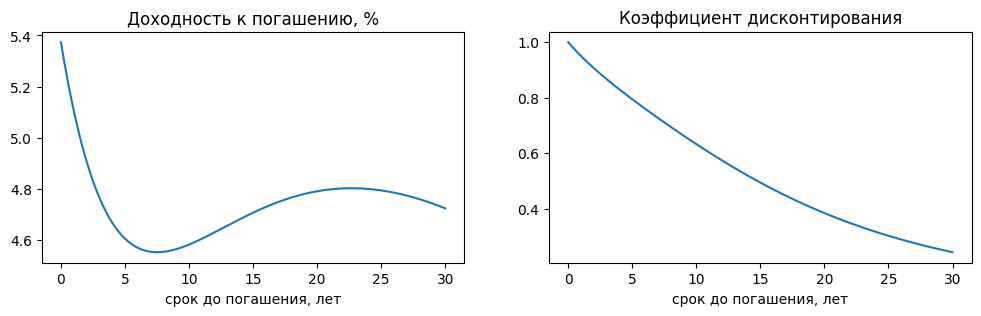
\includegraphics[width=\textwidth]{pic/yield-curve.png}
\caption{Кривая бескупонной доходности в США. Данные на 24.04.2024.}
\label{11:f:zcb}
\end{figure}


\subsection{\difficult\ Численный алгоритм}
\label{iv:ss:algorithm}
В этом разделе мы опишем численный метод решения уравнения \eqref{iv:equation}, основанный на идеях статьи \cite{Jaeckel06}.
В его основе лежит классический итерационный метод Ньютона нахождения корня уравнения, причем будет показано, что он гарантированно сходится при специальном выборе начального приближения. 

Для начала приведем уравнение \eqref{iv:equation} к более удобному виду.
Будем считать, что $T>0$.
Пусть $V$ обозначает цену опциона колл или пут (в зависимости от того, какой из них рассматривается).
Введем обозначения
\[
y = \ln\frac FK, \qquad
p = \frac{V}{B\sqrt{FK}}, \qquad
x = \hat\sigma\sqrt{T},\qquad
\theta=\begin{cases}
  1 &\text{для опциона колл},\\
  -1 &\text{для опциона пут}.
\end{cases}
\]
Подставляя эти обозначения в формулу Блэка, можно переписать уравнение \eqref{iv:equation} так:
\begin{equation}
\label{11:black}
\theta\left(e^{\frac y2}\Phi\left(\theta\left(\frac yx + \frac x2\right)\right) - e^{-\frac y2}\Phi\left(\theta \left(\frac yx - \frac x2\right)\right)\right) - p=0.
\end{equation}
Также нетрудно преобразовать условие предложения \ref{iv:p:existence} и получить, что решение уравнения \eqref{11:black} существует и единственно тогда и только тогда, когда
\begin{equation}
\label{11:exist}
\theta \I(\theta y>0) (e^{\frac y2} - e^{-\frac y2}) < p < e^{\theta \frac y2}.
\end{equation}

Если выполнено условие \eqref{11:exist}, то можно найти $\hat\sigma$ численно.
Напомним, что общий метод Ньютона численного решения уравнения $f(x) = 0$ состоит в построении последовательности приближений $x_n$ таких, что при некоторых условиях на функцию $f$ имеет место сходимость $x_n\to x^*$, где $x^*$ "--- решение.

Начальное приближение $x_0$ выбирается произвольно (но от его выбора может зависеть сходимость метода).
Следующие приближения находятся по формуле
\[
x_{n+1} = x_n - \frac{f(x_n)}{f'(x_n)}.
\]
Смысл метода Ньютона в том, что в точке $x_n$ строится касательная к графику функции $f$, и новое приближение $x_{n+1}$ выбирается как точка пересечения этой касательной с осью абсцисс.
Обычно прекращают итерации, когда разность $|x_{n+1}-x_n|$ становится меньше заданной точности.
На рис.~\ref{iv:f:newton} изображен пример итераций метода Ньютона.

\begin{figure}[h]
\centering
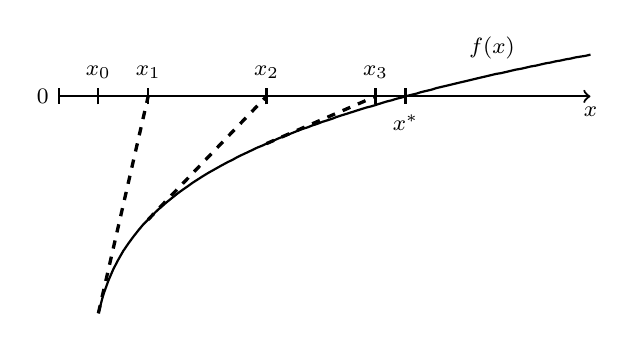
\begin{tikzpicture}[xscale=2.5,yscale=5]
\draw[thick,->] (-0.2,0) node[left] {\footnotesize $0$} --(2.5,0) node[below] {\footnotesize $x$};
\draw[thick] (-0.2,0.02)--(-0.2,-0.02);
\draw[thick] (0,-0.02) -- (0,0.02) node[above] {\footnotesize $x_0$};
\draw[thick] (0.253,-0.02) -- (0.253,0.02)  node[above] {\footnotesize $x_1$};
\draw[thick] (0.854,-0.02) -- (0.854,0.02) node[above] {\footnotesize $x_2$};
\draw[thick] (1.408,-0.02) -- (1.408,0.02) node[above] {\footnotesize $x_3$};
\draw[thick] (1.5605,0.02) -- (1.5605,-0.02) node[below] {\footnotesize $x^*$};
\draw (2,0.07) node[above] {\footnotesize $f(x)$};
% f(x) = (x+0.05)**0.2-1.1, x \in [0, 2.5]
\draw[thick] (0.000,-0.551)--(0.025,-0.504)--(0.051,-0.468)--(0.076,-0.439)--(0.101,-0.415)--(0.126,-0.393)--(0.152,-0.374)--(0.177,-0.357)--(0.202,-0.341)--(0.227,-0.326)--(0.253,-0.313)--(0.278,-0.300)--(0.303,-0.288)--(0.328,-0.277)--(0.354,-0.266)--(0.379,-0.256)--(0.404,-0.246)--(0.429,-0.237)--(0.455,-0.228)--(0.480,-0.219)--(0.505,-0.211)--(0.530,-0.203)--(0.556,-0.195)--(0.581,-0.188)--(0.606,-0.181)--(0.631,-0.174)--(0.657,-0.167)--(0.682,-0.161)--(0.707,-0.154)--(0.732,-0.148)--(0.758,-0.142)--(0.783,-0.136)--(0.808,-0.130)--(0.833,-0.125)--(0.859,-0.119)--(0.884,-0.114)--(0.909,-0.108)--(0.934,-0.103)--(0.960,-0.098)--(0.985,-0.093)--(1.010,-0.088)--(1.035,-0.083)--(1.061,-0.079)--(1.086,-0.074)--(1.111,-0.070)--(1.136,-0.065)--(1.162,-0.061)--(1.187,-0.057)--(1.212,-0.052)--(1.237,-0.048)--(1.263,-0.044)--(1.288,-0.040)--(1.313,-0.036)--(1.338,-0.032)--(1.364,-0.028)--(1.389,-0.025)--(1.414,-0.021)--(1.439,-0.017)--(1.465,-0.013)--(1.490,-0.010)--(1.515,-0.006)--(1.540,-0.003)--(1.566,0.001)--(1.591,0.004)--(1.616,0.007)--(1.641,0.011)--(1.667,0.014)--(1.692,0.017)--(1.717,0.021)--(1.742,0.024)--(1.768,0.027)--(1.793,0.030)--(1.818,0.033)--(1.843,0.036)--(1.869,0.039)--(1.894,0.042)--(1.919,0.045)--(1.944,0.048)--(1.970,0.051)--(1.995,0.054)--(2.020,0.057)--(2.045,0.059)--(2.071,0.062)--(2.096,0.065)--(2.121,0.068)--(2.146,0.070)--(2.172,0.073)--(2.197,0.076)--(2.222,0.078)--(2.247,0.081)--(2.273,0.084)--(2.298,0.086)--(2.323,0.089)--(2.348,0.091)--(2.374,0.094)--(2.399,0.096)--(2.424,0.099)--(2.449,0.101)--(2.475,0.103)--(2.500,0.106);
%
\draw[very thick,dashed] (0.000, -0.551) -- (0.253,0);
\draw[very thick,dashed] (0.253, -0.313) -- (0.854,0);
\draw[very thick,dashed] (0.854, -0.120) -- (1.408,0);
\end{tikzpicture}
\caption{Решение уравнения методом Ньютона.}
\label{iv:f:newton}
\end{figure}

\begin{proposition}
\label{iv:p:newton}
Предположим, что функция $f(x)$ непрерывно дифференцируема, строго возрастает и вогнута на  отрезке $[x_0,x^*]$, где $f(x^*)=0$. 
Тогда метод Ньютона с начальным приближением $x_0$ сходится к $x_*$.

Аналогичное утверждение верно, если $f$ выпукла на отрезке $[x^*,x_0]$.
\end{proposition}

\begin{proof}
Докажем только первое утверждение; второе аналогично.
В силу возрастания $f$, имеем $f(x_0) < 0$.
Так как график вогнутой функции лежит ниже любой своей касательной, то касательная, проведенная в точке $x_0$, должна пересечь ось абсцисс между точками $x_0$ и $x_*$.
Используя то же самое рассуждение, по индукции получаем, что $x_{n-1} < x_n < x_*$ для всех $n$.

Таким образом, последовательность $x_n$ возрастает и ограничена сверху значением $x_*$.
Следовательно, она имеет предел $\tilde x$.
Покажем, что $\tilde x=x_*$.
Предположим, от противного, что $\tilde x < x_*$.
Тогда найдутся такие $\epsilon,\delta>0$, что $f(x)/f'(x) \le -\epsilon$ при $x \in (\tilde x, \tilde x+\delta)$ (в силу того, что $f(x)$ отрицательна в окрестности $\tilde x$, а $f'(x)$ ограничена и положительна в силу своей непрерывности и возрастания $f(x)$).
Но так как $x_{n+1} - x_n = -f(x_n)/f'(x_n)$, то получаем противоречие со сходимостью последовательности $x_n$. Значит, $\tilde x = x_*$.  
\end{proof}

\begin{proposition}
Пусть выполнено условие \eqref{11:exist}.
Обозначим за $x^*$ решение уравнения \eqref{11:black}.
Тогда справедливы следующие утверждения.

1. Если $y=0$ (опцион ATMF), то 
\begin{equation}
\label{11:atm}
x^* = 2 \Phi^{-1}\left(\frac{1+p}{2}\right),
\end{equation}
где $\Phi^{-1}$ "--- обратная к стандартной нормальной функции распределения.

2. Если $y\neq 0$, то правая часть уравнения \eqref{11:black}, рассматриваемая как функция от $x$, имеет точку перегиба $x_0 = \sqrt{2|y|}$ и является выпуклой на интервале $(0,x_0)$ и вогнутой на $(x_0,\infty)$, а метод Ньютона с начальным приближением $x_0 = \sqrt{2|y|}$ сходится к $x^*$.
\end{proposition}

\begin{proof}
Формула \eqref{11:atm} очевидно следует из подстановки $y=0$ в \eqref{11:black}.
Докажем второе утверждение.
Обозначим за $f(x)$ правую часть \eqref{11:black}.
Непосредственно вычисляется
\[
f'(x) = \frac{1}{\sqrt{2\pi}} e^{-\frac12\left(\frac{y^2}{x^2} + \frac{x^2}4\right)},\qquad
f''(x) = \frac{x}{\sqrt{2\pi}} e^{-\frac12\left(\frac{y^2}{x^2} + \frac{x^2}4\right)}
  \left(\frac{y^2}{x^4} - \frac14\right).
\]
Видно, что $f'>0$, и, следовательно, $f$ строго возрастает.
Кроме того, $f''(x) > 0$ при $x < x_0$ и $f''(x) < 0$ при $x > x_0$.
Таким образом, $f$ выпукла на $(0,x_0]$ и вогнута на $[x_0,\infty)$.

Пусть $x_0$ используется в качестве начального приближения метода Ньютона.
Если $f(x_0) < 0$, то $x_0$ лежит слева от корня $x^*$, и можно воспользоваться первым утверждением предложения \ref{iv:p:newton}, что гарантирует сходимость метода Ньютона.
Аналогично, если $f(x_0) > 0$, то $x_0$ лежит справа от $x^*$, и можно воспользоваться вторым утверждением.
\end{proof}

Итак, из приведенных рассуждений следует, что для нахождения подразумеваемой волатильности нужно решить уравнение \eqref{11:black} и  положить $\hat\sigma = x^*/\sqrt{T}$, где $x^*$ "--- решение уравнения. 




\summary
\begin{itemize}
\item Подразумеваемая волатильность $\hat\sigma$ "--- это значение параметра $\sigma$, при котором цена конкретного опциона в модели \bs\ (вычисленная по формуле Блэка) совпадает с его рыночной ценой.

\item Подразумеваемая волатильность на практике оказывается разной для опционов с различными страйками и временем экспирации, что, в частности, говорит о том, что модель \bs\ не может правильно описать реальные рыночные данные (в ней подразумеваемая волатильность всегда постоянна).

\item Поверхностью волатильности называют график функции $\hat\sigma(T,K)$, а улыбкой "--- одно его сечение при фиксированном $T$.

\item Для построения поверхности подразумеваемой волатильности используют цены опционов ATMF и OTMF, форвардные цены вычисляют из паритета цен опционов колл-пут, а дисконтирующие коэффициенты "--- из кривой доходности государственных облигаций (если нет более подходящих данных).
\end{itemize}
